\section{跨边界延拓}
\label{sec:sobolev-extension}

许多论证希望在全空间$\mathbb R^d$上进行，那里磨光不受边界限制，平移和缩放也可以自由使用。为此要把区域$\Omega$上的Sobolev函数延拓成全空间上的Sobolev函数，并且延拓后的范数受原范数控制。这和把一段向量补长不同：补上去的部分不能破坏弱导数的存在。本节先在平直边界附近用反射说明函数怎样越过边界，再在有界Lipschitz区域上陈述一般的延拓定理，并由此得到光滑到边界的逼近。

\paragraph{一维反射}
设$f\in W^{1,p}(0,1)$，$1\leq p<\infty$。由第~\ref{chap:smoothing-weak-derivatives}章，$f$有绝对连续代表，仍记为$f$。在$(-1,1)$上令$Ef(x)=f(|x|)$。它在$[-1,0]$和$[0,1]$上分别绝对连续，并在$x=0$处取同一个值$f(0)$，所以在$[-1,1]$上绝对连续，几乎处处导数为$\operatorname{sgn}(x)f'(|x|)$。

绝对连续函数的几乎处处导数就是它的弱导数，因此$Ef\in W^{1,p}(-1,1)$。两侧对称，范数正好翻倍：
\begin{equation}
\lVert Ef\rVert_{W^{1,p}(-1,1)}^p=2\lVert f\rVert_{W^{1,p}(0,1)}^p .
\label{eq:sobolev-reflection-norm}
\end{equation}
用$f(x)=1+x-x^2$手算一次。$p=2$时，
\[
\int_0^1f^2\,\mathrm dx=\frac{41}{30},\qquad
\int_0^1(f')^2\,\mathrm dx=\int_0^1(1-2x)^2\,\mathrm dx=\frac13,
\]
所以$\lVert f\rVert_{H^1(0,1)}^2=17/10$，延拓后是$17/5$。

图~\ref{fig:sobolev-reflections}的(a)画的就是这个偶反射。反射在原点通常产生一个折点，正如$|x|$那样，但折点不破坏一阶弱导数的存在，因为两侧的值连在一起。

\begin{BookInlineFigure}
  \centering
  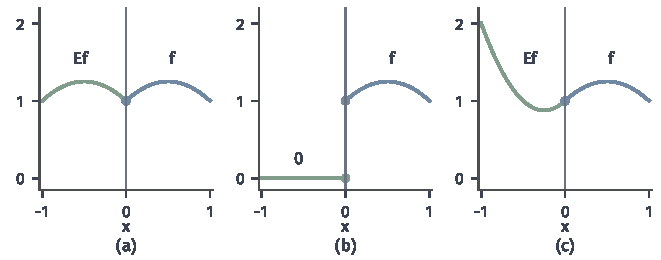
\includegraphics[width=112mm]{figures/04-spaces-measures-and-geometry/03-function-spaces/matplotlib/sobolev-reflections/figure.pdf}
  \caption{同一函数$f(x)=1+x-x^2$的三种延拓，蓝色为原函数，绿色为$x<0$一侧补上的部分。(a)偶反射，在原点连续，但有折点，属于$H^1$，一般不属于$H^2$。(b)零延拓，在原点跳跃，不属于$H^1$。(c)二阶反射$Ef(x)=-3f(-x)+4f(-x/2)$，在原点函数值和一阶导数都相接，属于$H^2$。}
  \label{fig:sobolev-reflections}
\end{BookInlineFigure}

\paragraph{半空间上的偶反射}
高维时最简单的边界是超平面。记$\mathbb R^d_+$为$x_d>0$的半空间，点写成$x=(x',x_d)$，其中$x'\in\mathbb R^{d-1}$。设$f$在闭半空间上连续可微、支撑有界，作偶反射
\[
Ef(x',x_d)=f(x',|x_d|).
\]
我们验证它在全空间有弱导数。对$i<d$，反射不涉及$x_i$，在两个半空间内分别分部积分，就得到$\partial_iEf(x',x_d)=(\partial_if)(x',|x_d|)$。

对$i=d$，取测试函数$\varphi\in C_c^\infty(\mathbb R^d)$，固定$x'$，分别在$x_d>0$和$x_d<0$上对$x_d$分部积分：
\[
\begin{aligned}
\int_0^\infty f(x',t)\,\partial_d\varphi\,\mathrm dt
&=-f(x',0)\varphi(x',0)-\int_0^\infty\partial_df\,\varphi\,\mathrm dt,\\
\int_{-\infty}^0 f(x',-t)\,\partial_d\varphi\,\mathrm dt
&=f(x',0)\varphi(x',0)+\int_{-\infty}^0(\partial_df)(x',-t)\,\varphi\,\mathrm dt .
\end{aligned}
\]
第二式用了链式法则：$t\mapsto f(x',-t)$的导数是$-(\partial_df)(x',-t)$。

两式相加，边界面上的项$\pm f(x',0)\varphi(x',0)$恰好相消。再对$x'$积分，得
\[
\int_{\mathbb R^d}Ef\,\partial_d\varphi\,\mathrm dx
=-\int_{\mathbb R^d}\operatorname{sgn}(x_d)\,(\partial_df)(x',|x_d|)\,\varphi\,\mathrm dx .
\]
所以
\[
\partial_dEf=\operatorname{sgn}(x_d)\,(\partial_df)(x',|x_d|).
\]
两侧对称，范数恒等式与式~\eqref{eq:sobolev-reflection-norm}相同：全空间上的$p$次方范数是半空间上的两倍。

上面的计算要求$f$光滑到边界并且支撑有界，一般的$f\in W^{1,p}(\mathbb R^d_+)$（$1\leq p<\infty$）可以这样逼近。先用$\chi(x/R)$截断，由引理~\ref{lem:sobolev-product-rule}和控制收敛，$R\to\infty$时误差趋于零。再向内部平移，$f_h(x',x_d)=f(x',x_d+h)$在更大的半空间$x_d>-h$上有定义，用半径小于$h$的磨光，就得到在闭半空间上光滑、支撑有界的函数。令$h$与磨光半径趋于零，由平移的积分连续性和磨光收敛，这些函数在$W^{1,p}(\mathbb R^d_+)$中趋于截断后的函数。

于是$E$在一个稠密子空间上满足上述范数恒等式。由$W^{1,p}(\mathbb R^d)$的完备性，它唯一地延伸为整个$W^{1,p}(\mathbb R^d_+)$上的有界线性算子，延伸后的$Ef$仍几乎处处等于$f(x',|x_d|)$。

\paragraph{零延拓与边界相容条件}
与偶反射对照，把$f$在$x_d<0$处直接补成零，称为\term{零延拓}（zero extension）。重做上面的分部积分，只剩$x_d>0$一侧，边界项
\[
-\int_{\mathbb R^{d-1}}f(x',0)\,\varphi(x',0)\,\mathrm dx'
\]
不再被抵消。若$f$在边界面上的值不恒为零，这一项集中在零测的超平面上，不能写成$\int g\varphi$的形式，论证与阶跃函数相同。图~\ref{fig:sobolev-reflections}的(b)是一维的情形：跳跃出现在接缝处，$(0,1)$上的常数$1$零延拓后就是阶跃函数，不属于$W^{1,p}(-1,1)$。

所以零延拓需要边界相容条件：函数在边界上的值为零。对光滑到边界的函数，这一条件可以逐点检查。对一般的Sobolev函数，“边界值”要通过第~\ref{sec:sobolev-trace}小节的迹来理解。第~\ref{sec:sobolev-compact-closure}小节的闭包空间恰好由这类函数组成，零延拓在其上保持范数不变。

\paragraph{高阶延拓}
偶反射对$W^{2,p}$不够。反射后$\partial_dEf$在$x_d>0$一侧趋于$\partial_df(x',0)$，在另一侧趋于$-\partial_df(x',0)$。只要法向导数在边界上不为零，$\partial_dEf$就有跳跃，没有局部可积的弱导数。高阶延拓必须让函数及其直到$k-1$阶的法向导数在边界两侧相接。

对$k=2$，可以在$x_d<0$处令
\begin{equation}
Ef(x',x_d)=-3f(x',-x_d)+4f\Bigl(x',-\frac{x_d}{2}\Bigr).
\label{eq:sobolev-second-order-reflection}
\end{equation}
系数的选取是为了让两个条件同时成立。在$x_d=0$处，函数值为$-3f+4f=f(x',0)$。对$x_d$求导，得到
\[
\partial_dEf(x',x_d)=3\,\partial_df(x',-x_d)-2\,\partial_df\Bigl(x',-\frac{x_d}2\Bigr),
\]
它在边界上等于$\partial_df(x',0)$。

用图~\ref{fig:sobolev-reflections}(c)的函数手算核对。$f(x)=1+x-x^2$代入式~\eqref{eq:sobolev-second-order-reflection}，$x<0$时得
\[
Ef(x)=-3(1-x-x^2)+4\Bigl(1-\frac x2-\frac{x^2}4\Bigr)=1+x+2x^2 .
\]
在$x=0$处函数值都是$1$，一阶导数都是$1$。二阶导数左侧是$4$，右侧是$-2$，有跳跃，但二阶导数只需要作为$L^p$函数存在。

一般地，$Ef$在全空间连续可微，两侧分别二阶光滑，按前面的分部积分，二阶弱导数存在且局部可积。$x_d<0$一侧的各阶导数是$f$的导数在两个缩放位置的有限组合，换元后得到
\[
\lVert Ef\rVert_{W^{2,p}(\mathbb R^d)}\leq C\lVert f\rVert_{W^{2,p}(\mathbb R^d_+)} .
\]
对一般的$k$，取$k$个系数使前$k$个法向导数都相接即可。

\paragraph{Lipschitz区域}
一般区域的边界可以弯曲，甚至有棱角。只要边界在每点附近都能写成函数图像，并且区域只位于图像的一侧，就可以在局部把边界拉直，再用反射。

\begin{definition}[Lipschitz区域]
\label{def:sobolev-lipschitz-domain}
称有界开集$\Omega\subset\mathbb R^d$为\term{Lipschitz区域}（Lipschitz domain），若对每个$x_0\in\partial\Omega$，存在$r>0$、经旋转与平移得到的坐标$(x',x_d)$以及Lipschitz函数$\gamma:\mathbb R^{d-1}\to\mathbb R$，使
\begin{equation}
\Omega\cap B(x_0,r)=\{x\in B(x_0,r):x_d>\gamma(x')\}.
\label{eq:sobolev-lipschitz-graph}
\end{equation}
\end{definition}

图~\ref{fig:sobolev-lipschitz-domains}对比了三种情形。球、立方体和有界凸开集都是Lipschitz区域；立方体在棱角处不光滑，但把坐标轴转过去，局部仍是Lipschitz图像。挖去一条线段的圆盘不是：割缝两侧都属于区域，区域不能只位于割缝的一侧。

\begin{BookInlineFigure}
  \centering
  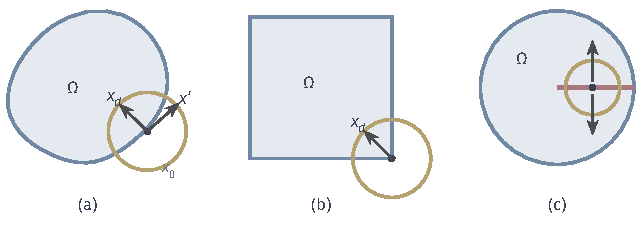
\includegraphics[width=108.356mm]{figures/04-spaces-measures-and-geometry/03-function-spaces/tikz/sobolev-lipschitz-domains/figure.pdf}
  \caption{Lipschitz区域的局部图像条件，黄圈为球$B(x_0,r)$。(a)弯曲边界，局部坐标中$x_d$指向区域内，$\Omega$位于图像$x_d=\gamma(x')$的上方。(b)方形的角点，把$x_d$轴转到对角线方向后，边界仍是Lipschitz图像。(c)割缝圆盘，红线为割缝，黄圈内区域同时位于割缝两侧，不能写成单侧图像，因而不是Lipschitz区域。}
  \label{fig:sobolev-lipschitz-domains}
\end{BookInlineFigure}

\begin{theorem}[Lipschitz区域上的延拓]
\label{thm:sobolev-extension}
设$\Omega\subset\mathbb R^d$为有界Lipschitz区域，$1\leq p<\infty$。存在有界线性算子$E:W^{1,p}(\Omega)\to W^{1,p}(\mathbb R^d)$和有界集合$B_\Omega$，使对每个$f\in W^{1,p}(\Omega)$，$Ef$在$\Omega$上几乎处处等于$f$，并且$Ef$在$B_\Omega$之外为零。
\end{theorem}

完整证明要处理Lipschitz变换下的弱导数，篇幅较长，读者可查阅Sobolev空间的专著，这里说明构造的步骤。边界是紧集，可以用有限个满足定义的球覆盖，再加上一个闭包含于$\Omega$的开集覆盖内部。取从属于这有限个开集的单位分解，把$f$分成有限块，内部那块在边界附近为零，直接零延拓。

每个边界块用变换$(x',x_d)\mapsto(x',x_d-\gamma(x'))$拉直为半空间上的函数，作偶反射，再变换回去。这个变换与它的逆都是Lipschitz映射，它们把$W^{1,p}$函数映为$W^{1,p}$函数，范数只相差由$\gamma$的Lipschitz常数决定的倍数。最后用一个固定的截断函数乘以和式，使所有延拓都在同一有界集合外为零。

这一构造对一阶空间有效，但不能直接推广到高阶：Lipschitz拉直变换只有一阶导数的控制，复合以后二阶导数一般不存在。若边界是$C^k$图像，可以用光滑的拉直变换配合上面的高阶反射。对一般有界Lipschitz区域，$W^{k,p}$的延拓也存在，但需要不同的构造，读者可查阅相关专著。

\paragraph{光滑到边界的逼近}
延拓定理的一个直接推论是更强的逼近：逼近函数可以取为全空间紧支撑光滑函数在$\Omega$上的限制，从而连同各阶导数都连续到边界。

\begin{theorem}[光滑到边界的逼近]
\label{thm:sobolev-smooth-up-to-boundary}
设$\Omega$为有界Lipschitz区域，$1\leq p<\infty$。则$\{\psi|_\Omega:\psi\in C_c^\infty(\mathbb R^d)\}$在$W^{1,p}(\Omega)$中稠密。
\end{theorem}

\begin{proof}
对$f\in W^{1,p}(\Omega)$，由定理~\ref{thm:sobolev-extension}得到在有界集合外为零的$Ef\in W^{1,p}(\mathbb R^d)$。$Ef*\rho_\varepsilon$光滑且支撑紧，由式~\eqref{eq:sobolev-whole-space-mollify}，它在$W^{1,p}(\mathbb R^d)$中趋于$Ef$。限制到$\Omega$上范数只会变小，所以
\[
\lVert(Ef*\rho_\varepsilon)|_\Omega-f\rVert_{W^{1,p}(\Omega)}
\leq\lVert Ef*\rho_\varepsilon-Ef\rVert_{W^{1,p}(\mathbb R^d)}\to0.
\qedhere
\]
\end{proof}

记这类限制函数的全体为$C^\infty(\overline\Omega)$。与定理~\ref{thm:sobolev-meyers-serrin}相比，这里多了边界正则性的假设，换来的是光滑到边界的逼近函数。下一节定义边界值时，正是先对这类函数直接限制到边界，再用逼近推广到整个空间。
